
\chapter{Introduction}

\minitoc{}
\bigskip

Ce premier chapitre introduit les infrastructures de collaboration. Il motive notre intérêt pour les infrastructures pair-à-pair de collaboration.
Il donne un aperçu de nos problématiques de recherche et de nos contributions.
Il détaille également l'organisation de ce manuscrit et il énumère nos publications.

\clearpage
\section{Contexte}

% Note : ne pas se centrer sur l'édition collaborative, mettre des exemples

%Internet est devenu une plate-forme où les utilisateur·ice·s et les services automatisés ne consultent plus uniquement des contenus, mais les produisent et les enrichissent collectivement.
%Les utilisateur·ice·s bénéficient de l'expérience de chacun·e.
%Les contenus produits sont plus élaborés et de meilleure qualité.
%
%Les applications de collaboration facilitent la production collaborative de contenus.
%Elles permettent à des collaborateur·ices géographiquement éloignés de contribuer à un même contenu.
%Elles permettent également de modifier simultanément ou de manière différée les contenus.
%Chaque contributeur·ice modifie individuellement un contenu partagé.
%Ses modifications sont à termes observées et prises en compte par les autres contributeur·ice·s.
%
%\begin{itemize}
%    \item Les éditeurs collaboratifs de texte permettent d'écrire en simultané.
%    \item Les réseaux sociaux permettent de partager et de commenter des contenus multimédias.
%\end{itemize}{}


%Les infrastructures de collaboration permettent à un groupe d'individus et de services automatisés de produire collectivement des contenus.

Internet est devenu une plate-forme où les internautes ne consultent plus uniquement des contenus, mais les produisent et les enrichissent collectivement~\autocite{mogan2010_web2groupware}~: elles et ils partagent et commentent des contenus multimédias au sein des réseaux sociaux~; elles et ils co-écrivent des documents à l'aide d'éditeurs collaboratifs~; elles et ils co-programment à l'aide de gestionnaires de versions.
Les productions de tels contenus sont le résultat d'activités de collaboration~\autocite{ellis1991_groupware} qui se répartissent dans l'espace et le temps.
Les contributeur·ices modifient individuellement un contenu partagé.
Elles et ils peuvent se trouver à des endroits géographiquement éloignés et peuvent modifier simultanément ou de manière différée les contenus partagés.
Leurs modifications sont à terme observées et prises en compte par les autres contributeur·ice·s.

% les systèmes centralisées

Les applications de collaboration ont permis l'émergence et la diffusion des activités de collaboration sur Internet.
Ces applications ont été initialement conçues sur des infrastructures centralisées.
Dans de telles infrastructures, les activités de collaboration s'organisent autour d'un serveur.
Les collaborateur·ice·s sont connecté·e·s les un·e·s aux autres à travers le serveur.
Toutes les modifications qu'elles et ils effectuent sur les contenus partagés sont relayées par le serveur aux autres collaborateur·ice·s.
Le serveur peut éventuellement transformer les modifications avant de les transmettre.
Dans la \autoref{fig:authority} les collaboratrices soumettent leur modification au serveur qui les appliquent sur le contenu.
Le serveur transmet la nouvelle version du contenu aux collaboratrices.
Le rôle prépondérant du serveur engendre plusieurs problèmes~:

\begin{figure}[hbt]
\centering
\begin{subfigure}{.5\linewidth}
    \centering
    \begin{tikzpicture}
        % devices
        \node[
            label=below:{Serveur}
        ](S){
\includegraphics[scale=0.8]{collab/cloud.pdf}};
        \path (S)
            to +(180:3.6) node[
                label=below:{Alice}
            ](A){
\includegraphics[scale=0.6]{collab/device.pdf}}
            to +(35:3.6) node[
                label=below:{Bea}
            ](B){
\includegraphics[scale=0.6]{collab/device.pdf}}
            to +(-35:3.6) node[
                label=below:{Carol}
            ](C){
\includegraphics[scale=0.6]{collab/device.pdf}};
        % Links
        \draw[link,-latex] (A) to node[near start]{
            
\includegraphics[scale=0.5]{collab/contrib-a1.pdf}
        } (S);
        \draw[link,-latex] (B.west) to node[near start]{
            
\includegraphics[scale=0.5]{collab/contrib-b1.pdf}
        } (S);
        \draw[link] (C.west) to (S);
    \end{tikzpicture}
    \caption{}\label{fig:authority-1}
\end{subfigure}%
\begin{subfigure}{.5\linewidth}
\centering
    \begin{tikzpicture}
        % devices
        \node[
            label=below:{Serveur}
        ](S){
\includegraphics[scale=0.8]{collab/cloud.pdf}};
        \path (S)
            to +(180:1.8) coordinate (Adoc)
            to +(180:3.6) node[
                label=below:{Alice}
            ](A){
\includegraphics[scale=0.6]{collab/device.pdf}}
            to +(35:1.8) coordinate (Bdoc)
            to +(35:3.6) node[
                label=below:{Bea}
            ](B){
\includegraphics[scale=0.6]{collab/device.pdf}}
            to +(330:1.8) coordinate (Cdoc)
            to +(-35:3.6) node[
                label=below:{Carol}
            ](C){
\includegraphics[scale=0.6]{collab/device.pdf}};
        % Links
        \draw[link,-latex] (S) to (A);
        \draw[link,-latex] (S) to (B.west);
        \draw[link,-latex] (S) to (C.west);
        % Msgs
        \node at (Adoc) {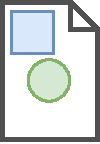
\includegraphics[scale=0.5]{collab/doc-a1-b1.pdf}};
        \node at (Bdoc) {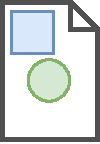
\includegraphics[scale=0.5]{collab/doc-a1-b1.pdf}};
        \node at (Cdoc) {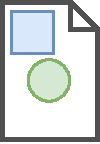
\includegraphics[scale=0.5]{collab/doc-a1-b1.pdf}};
    \end{tikzpicture}
    \caption{}\label{fig:authority-2}
\end{subfigure}
\caption[Activité de collaboration au sein d'une infrastructure centralisée]{Exemple d'une activité de collaboration au sein d'une infrastructure centralisée.
Alice, Bea, et Carol sont connectées à un serveur.
Elles éditent ensemble un dessin.
\subref{fig:authority-1} Alice et Bea souhaitent modifier le dessin partagé~: Alice souhaite ajouter un carré et Bea souhaite ajouter un cercle.
Elles soumettent leur modification au serveur.
\subref{fig:authority-2} Le serveur intègre leurs modifications et transmet la nouvelle version du dessin aux collaboratrices.}\label{fig:authority}
\end{figure}

\paragraph{Disponibilité.}
Toutes les modifications du contenu partagé sont transmises aux collaborateur·ice·s par l'intermédiaire du serveur.
L'indisponibilité du serveur rend impossible la collaboration.
Le serveur est un \emph{point unique de défaillance}~\autocite{dooley2001designing}.

\paragraph{Latence.}
Le traitement centralisé des modifications effectuées par les collaborateur·ice·s introduit des latences.
Ces latences, ajoutées à celles du réseau, peuvent être trop importantes pour la modification de contenu en simultané.
Nous parlons de simultané quand des collaborateur·ice·s éditent un même contenu au même moment et qu'elles et ils ont l'illusion de percevoir immédiatement les modifications de chacun·e.
\textcite{ignat_2015_user-and-delay} ont montré que les activités de collaboration en simultané étaient compromises lorsque le délai entre des modifications de contenu et leurs observations par les autres était trop important.
Ce délai engendre des conflits de modification sur le contenu partagé.
Les collaborateur·ice·s adoptent des stratégies qui limitent leurs interactions pour éviter ces conflits.
Ce qui réduit l'efficacité de la collaboration.
%Les latences doivent être suffisamment faibles pour prendre en compte les modifications des autres collaborateur·ice·s lorsque nous effectuons nos propres modifications.

\paragraph{Passage à l'échelle.}
Le serveur peut difficilement s'adapter à un accroissement du nombre de modifications et du nombre de collaborateur·ice·s.
Cette difficulté se traduit par une augmentation des latences pour intégrer de nouvelles modifications et propager les nouvelles versions du contenu partagé.
Elle peut également produire un déni de service qui rend indisponible le serveur.
Pour éviter ce problème les applications de collaboration limitent le nombre de collaborateur·ice·s autorisé·e·s au sein d'une collaboration~\autocite{ignat_2015_user-and-delay,ignat2014_delayeffect}.
Ils supportent pas ou difficilement les activités de collaboration qui impliquent un nombre important de collaborateur·ice·s.

%\paragraph{Coût.}
%Afin de réduire les latences introduites par les infrastructures centralisées et de supporter un nombre raisonnable de collaborateur·ice·s, le serveur est en général dotée d'une puissance de calcul conséquente.
%Cette puissance de calcul engendre des coût environnementaux et financiers.
%Ce qui se traduit également par le contrôle de telles infrastructures par des organisations qui disposent des ressources nécessaires à leur déploiement.

\paragraph{Confidentialité, Vie Privée, et Censure.}
Le rôle de carrefour du serveur permet la collecte massive de données privées et confidentielles, ainsi que le contrôle systématique de l'information et donc de son éventuelle censure \autocite{jard2016_langage}.

\paragraph{Sécurité.}
Le rôle central du serveur en fait une cible privilégiée d'attaque \autocite{jard2016_langage}.
La corruption du serveur permet à l'attaquant d'accéder à de nombreuses données sensibles des utilisateur·ice·s et éventuellement de les altérer.

\paragraph{Propriété des contenus.}
Le serveur détient les contenus partagés.
Les collaborateur·ice·s perdent la propriété de leurs contenus et de leurs contributions.
Le serveur peut ainsi restreindre la modification et la consultation des contenus produits.
Il peut supprimer le contenu sans en alerter préalablement les contributeur·ice·s.

\paragraph{Modes de collaboration~\autocite{dourish_1995_divergence}.}
Les collaborateur·ice·s sont restreint·e·s dans les formes que peuvent prendre leur collaboration.
Les infrastructures centralisées leur permettent de contribuer depuis des endroits géographiquement éloignés et à des instants différents.
Toutefois elles et ils doivent être connecté·e·s au serveur.
Ils ne peuvent pas travailler en sous-groupes déconnecté·e·s les un·e·s des autres.
La modification hors ligne, voire la consultation hors ligne, des contenus partagés n'est pas toujours supportée.

\bigskip

%Son indisponibilité rend les collaborations impossibles.
%La serveur constitue donc un point unique de défaillance.
%Par ailleurs, les infrastructures centralisées passent difficilement à l'échelle.
%Elles peuvent souffrir de latence trop importante pour la modification de contenu en simultané.
%\textcite{ignat_2015_user-and-delay} ont en effet montré que les activités de collaboration en simultané étaient compromises lorsque le délai entre des modifications de contenu et leurs observations par les autres était trop important.
%
%Au-delà de leurs limitations techniques, les infrastructures centralisés soulèvent des questionnement éthiques.
%Le rôle de carrefour du serveur permet la collecte massive de données privées et confidentielles, ainsi que le contrôle systématique de l'information et donc de son éventuelle censure.
%Ces comportements peuvent être menés par l'organisation qui contrôle et maintient l'infrastructure ou par un attaquant.
%Se pose également la question de la propriété des contenus produits.

% les infrastructures pair-à-pair de collaboration

\begin{figure}[t]
\centering
\begin{subfigure}{.5\linewidth}
    \centering
    \begin{tikzpicture}
        % devices
        \path (0,0)
            to +(190:2) node[
                label=below:{Alice},
                label=left:{
\includegraphics[scale=0.5]{collab/doc-a1.pdf}}
            ](A){
\includegraphics[scale=0.6]{collab/device.pdf}}
            to +(70:2) node[
                label=above:{Bea},
                label=right:{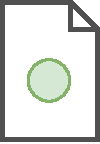
\includegraphics[scale=0.5]{collab/doc-b1.pdf}}
            ](B){
\includegraphics[scale=0.6]{collab/device.pdf}}
            to +(-50:2) node[
                label=below:{Carol},
                label=right:{
\includegraphics[scale=0.5]{collab/doc.pdf}}
            ](C){
\includegraphics[scale=0.6]{collab/device.pdf}};
        % Links
        \draw[link] (A) to (B);
        \draw[link] (B) to (C);
        \draw[link] (C) to (A);
    \end{tikzpicture}
    \caption{}\label{fig:optimisqtic-replciation-scenario-1}
\end{subfigure}%
\begin{subfigure}{.5\linewidth}
\centering
    \begin{tikzpicture}
        % devices
        \path (0,0)
            to +(190:2) node[
                label=below:{Alice},
                label=left:{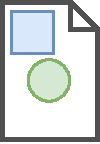
\includegraphics[scale=0.5]{collab/doc-a1-b1.pdf}}
            ](A){
\includegraphics[scale=0.6]{collab/device.pdf}}
            to +(70:2) node[
                label=above:{Bea},
                label=right:{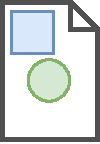
\includegraphics[scale=0.5]{collab/doc-a1-b1.pdf}}
            ](B){
\includegraphics[scale=0.6]{collab/device.pdf}}
            to +(-50:2) node[
                label=below:{Carol},
                label=right:{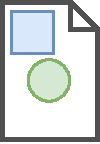
\includegraphics[scale=0.5]{collab/doc-a1-b1.pdf}}
            ](C){
\includegraphics[scale=0.6]{collab/device.pdf}};
        % Links
        \draw[link] (A) to node[midway]{
\includegraphics[scale=0.5]{collab/sync.pdf}} (B);
        \draw[link] (B) to node[midway]{
\includegraphics[scale=0.5]{collab/sync.pdf}} (C);
        \draw[link] (C) to node[midway]{
\includegraphics[scale=0.5]{collab/sync.pdf}} (A);
    \end{tikzpicture}
    \caption{}\label{fig:optimisqtic-replciation-scenario-2}
\end{subfigure}
\caption[Activité de collaboration au sein d'une infrastructure pair-à-pair]{Exemple d'une activité de collaboration au sein d'une infrastructure pair-à-pair.
Alice, Bea, et Carol répliquent de manière optimiste un dessin.
Elles disposent chacune d'une copie du dessin.
\subref{fig:optimisqtic-replciation-scenario-1} Alice et Bea modifient indépendamment leur copie du dessin.
Alice ajoute un carré, alors que Bea ajoute un cercle.
Les copies des collaboratrices divergent~: les collaboratrices ont des dessins différents.
\subref{fig:optimisqtic-replciation-scenario-2} Elles synchronisent ensuite leurs copies afin d'intégrer les modifications de chacune.
Les copies convergent~: elles obtiennent ainsi le même dessin.}\label{fig:optimisqtic-replciation-scenario}
\end{figure}

La diffusion des activités de collaboration a inspiré de nouveaux usages qui poussent les infrastructures centralisées à leurs limites.
Par exemple, la prise de note en simultané durant un cours en ligne peut faire intervenir une promotion entière d'étudiant·e·s.
Ces usages se sont renforcés avec la crise sanitaire provoquée par la pandémie de \emph{COVID-19}.

Pour supporter ces nouveaux usages, plusieurs initiatives ont vu le jour~\autocite{benet2014ipfs,wood2014ethereum,mansour2016demonstration}.
Elles s'appuient sur des infrastructures pair-à-pair pour décentraliser les applications de collaboration.
Les infrastructures pair-à-pair de collaboration sont caractérisées par l'absence de serveur central.
Les appareils des collaborateur·ice·s sont des pairs.
Ils sont directement connectés les uns aux autres et partagent les mêmes responsabilités\footnote{Certaines infrastructures présentent des pairs privilégiés avec des responsabilités supplémentaires.%L'infrastructure reste décentralisée car plusieurs pairs peuvent avoir les mêmes privilèges.
}.

Les infrastructures pair-à-pair de collaboration visent la conception d'applications de collaboration hautement disponibles, aux latences faibles, qui tolèrent les partitions réseaux, et passent à l'échelle~\autocite{rodrigues2010peer}.
Pour ce faire, elles reposent sur la réplication optimiste des contenus~\autocite{saito_2005_optimisticreplication}.
Chaque pair possède une copie des contenus partagés.
Il interroge et modifie directement sa copie sans se coordonner avec les autres pairs.
Les modifications sont propagées en arrière plan aux autres pairs.
%Elles sont transmises immédiatement ou ultérieurement.
%Ce choix est laissé à la discrétion du protocole de réplication.
Les pairs intègrent à leur copie les modifications qu'ils reçoivent.
La \autoref{fig:optimisqtic-replciation-scenario} illustre un scénario de réplication optimiste.

%Le support de collaboration qui implique un grand nombre de collaborateur·ice·s augmente le risque d'apparition de latences et de comportements mal-intentionnés.
%Ce qui nous amène à questionner le passage à l'échelle et la sécurité des protocoles de réplication optimiste de contenu partagé.
%Nous détaillons ces aspects dans la \autoref{sec:problematic}.

Les infrastructures pair-à-pair de collaboration donne plus de responsabilités aux pairs.
Des collaborateur·ice·s peuvent davantage nuire au bon déroulement de la collaboration.
Les infrastructures pair-à-pair permettent également la participation d'un plus grand nombre de collaborateur·ice·s.
Ce qui nous amène à questionner la sécurité et le passage à l'échelle des protocoles de réplication optimiste.


\section{Problématiques et contributions}\label{sec:problematic}

%Les infrastructures pair-à-pair de collaboration permettent d'envisager la conception d'applications hautement disponible, aux latences faibles, et qui passent à l'échelle.

\subsection{Convergence en présence de pairs mal-intentionnés}

Les infrastructures pair-à-pair de collaboration permettent aux pairs de modifier en parallèle un contenu partagé.
Pour ce faire, les pairs répliquent le contenu partagé et modifient leur copie respective.
La modification concurrente du contenu engendre inévitablement la divergence des copies du contenu partagé~\autocite{dourish_1995_divergence}.
Dans la \autoref{fig:optimisqtic-replciation-scenario}, les copies divergent avant leur synchronisation.
Les protocoles de réplication optimiste sont responsables de la réconciliation de l'état des copies pour les faire converger vers un état qui intègre les modifications de chacun.
La convergence des copies conditionne la vivacité et donc le succès d'une collaboration.
Si deux contributeur·ice·s ont des copies qui ne sont pas capables de converger, leur vue du contenu sera différente.
Cette divergence de vue peut compromettre leur collaboration.
Assurer à terme la convergence des copies est donc important dans une infrastructure de collaboration.

Pour illustrer l'importance de la convergence, nous prenons l'exemple de l'organisation d'un événement festif ou politique.
Plusieurs réunions d'organisation ont lieu avant l'évènement.
Pour garder une trace de ces réunions et informer les bénévoles absents, les organisatrices de l'événement ont mis en place un document textuel partagé.
Les organisatrices et les bénévoles prennent collectivement des notes durant les réunions.
Ce document peut par exemple inclure des dates de rendez-vous pour préparer l'événement.
Si les pairs ne sont pas capables de converger, certains bénévoles risquent de manquer des rendez-vous essentiels.
Ce qui pourrait retarder, voire empêcher, la tenue de l'événement.

Certains pairs peuvent trouver un intérêt à compromettre le succès d'une collaboration.
Dans le cas de l'exemple précédent, il peut s'agir d'un opposant à la tenue de l'événement.
Nous nous intéressons en particulier aux pairs qui entreprennent des actions pour faire diverger de manière permanente la vue des autres pairs.
Ces pairs \emph{mal-intentionnés} cherchent donc à faire diverger de manière permanente les copies des autres pairs que nous qualifions d'\emph{honnêtes}.
Pour ce faire, les pairs mal-intentionnés utilisent les faiblesses de certains protocoles de réplication~: ils transmettent à différents pairs honnêtes des modifications distinctes qui sont perçues comme identiques par le protocole.
Il s'agit d'une \emph{équivoque}.
Par exemple, l'opposant à l'événement peut infiltrer le groupe de bénévoles et faire en sorte que les bénévoles observent différentes dates de rendez-vous de préparation de l'événement.
L'opposant répandrait ainsi la confusion et provoquerait l'absence de bénévoles à certains rendez-vous.
La \autoref{fig:equivocation-scenario} illustre un scénario dans lequel un pair mal-intentionné effectue une équivoque.
Les pairs honnêtes ne détectent pas l'équivoque.
Leurs copies divergent de manière permanente.

\paragraph{}Ce qui nous amène à formuler notre première question de recherche~: \textbf{Est-il possible d'assurer la convergence des copies des pairs honnêtes en présence de pairs mal-intentionnés et de conserver les propriétés offertes par les infrastructures pair-à-pair de collaboration~?}

\clearpage % better layout

\begin{figure}[hbt]
\centering
\begin{subfigure}{.5\linewidth}
    \centering
    \begin{tikzpicture}
        % devices
        \path (0,0)
            to +(190:2) node[
                label=below:{Alice},
                label=left:{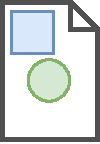
\includegraphics[scale=0.5]{collab/doc-a1-b1.pdf}}
            ](A){
\includegraphics[scale=0.6]{collab/device.pdf}}
            to +(70:2) node[
                label=above:{Bea},
                label=right:{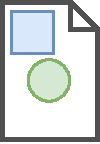
\includegraphics[scale=0.5]{collab/doc-a1-b1.pdf}}
            ](B){
\includegraphics[scale=0.6]{collab/device.pdf}}
            to +(-50:2) node[
                label=below:{Mallory}
            ](M){
\includegraphics[scale=0.6]{collab/device-malicious.pdf}};
        % Links
        \draw[link] (A) to (B);
        \draw[link,-latex] (M) to node[near start]{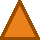
\includegraphics[scale=0.5]{collab/contrib-m1.pdf}} (A);
        \draw[link,-latex] (M) to node[near start]{
\includegraphics[scale=0.5]{collab/contrib-m1p.pdf}} (B);
    \end{tikzpicture}
    \caption{}\label{fig:equivocation-scenario-1}
\end{subfigure}%
\begin{subfigure}{.5\linewidth}
\centering
    \begin{tikzpicture}
        % devices
        \path (0,0)
            to +(190:2) node[
                label=below:{Alice},
                label=left:{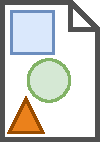
\includegraphics[scale=0.5]{collab/doc-a1-b1-m1.pdf}}
            ](A){
\includegraphics[scale=0.6]{collab/device.pdf}}
            to +(70:2) node[
                label=above:{Bea},
                label=right:{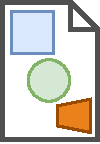
\includegraphics[scale=0.5]{collab/doc-a1-b1-m1p.pdf}}
            ](B){
\includegraphics[scale=0.6]{collab/device.pdf}}
            to +(-50:2) node[
                label=below:{Mallory}
            ](M){
\includegraphics[scale=0.6]{collab/device-malicious.pdf}};
        % Links
        \draw[link] (A) to node[midway]{
\includegraphics[scale=0.5]{collab/sync.pdf}} (B);
        \draw[link] (M) to (A);
        \draw[link] (M) to (B);
    \end{tikzpicture}
    \caption{}\label{fig:equivocation-scenario-2}
\end{subfigure}
\caption[Équivoque]{Exemple d'une équivoque qui vise à faire diverger de manière permanente les copies des collaboratrices honnêtes.
Alice et Bea sont honnêtes.
Elles répliquent de manière optimiste un dessin.
Mallory est mal-intentionnée.
Elle souhaite compromettre la collaboration entre Alice et Bea.
\subref{fig:equivocation-scenario-1} Mallory effectue une équivoque.
Elle transmet à Alice l'ajout d'un triangle orange, alors qu'elle transmet à Bea l'ajout d'un trapèze orange.
Elle fait en sorte que ces modifications distinctes paraissent identique.
Par exemple, si l'on considère que la couleur est la seule information utilisée pour détecter la présence d'une forme sur le dessin, alors il n'est pas possible de différencier un dessin avec la première forme d'un dessin avec la seconde.
\subref{fig:equivocation-scenario-2} Alice et Bea intègrent la modification qu'elles reçoivent.
Leurs copies divergent.
Elles se synchronisent ensuite, mais elles ne détectent pas la divergence de leur copie.
L'objectif de Mallory est atteint~: les copies de Alice et Bea demeurent divergentes.}\label{fig:equivocation-scenario}
\end{figure}

De nombreux protocoles de réplication optimiste synchronisent les copies en échangeant des opérations~\autocite{baquero_2018_pure-op-crdt}.
L'opération synthétise une modification effectuée sur l'une des copies.
Un pair mal-intentionné met en oeuvre une équivoque en générant deux opérations distinctes mais qui sont perçues comme identiques par le protocole de réplication.
Pour détecter de telles opérations, les pairs peuvent utiliser des \emph{journaux authentifiés} d'opérations~\autocite{li_2004_sundr,mahajan_depot_2011,truong_authenticating_2012}.
Chaque pair possède un journal dans lequel il enregistre les opérations qu'il transmet et qu'il reçoit.
Chaque opération est signée par son auteur et référence des opérations sur-lesquelles elle dépend.
Deux opérations distinctes ont une signature différente.
Les pairs peuvent donc identifier les équivoques.
En considérant que le protocole de réplication puisse intégrer des opérations distinctes présentées comme identiques, les journaux authentifiés permettent donc d'assurer la convergence des copies des pairs honnêtes.

L'utilisation de journaux authentifiés représente un coût supplémentaire pour la collaboration.
Les pairs doivent conserver le journal, et donc l'ensemble des opérations qu'ils ont transmis et reçu.
Ce coût est en particulier visible lorsqu'un nouveau pair rejoint la collaboration.
Le nouveau pair doit en effet récupérer l'intégralité du journal pour obtenir l'état actuel du contenu partagé.
Au fur et à mesure de la collaboration, le journal croît.
Ce qui rend coûteux la transmission du journal et la construction de l'état actuel du contenu partagé à partir du journal.
L'utilisation de journaux authentifiés passe donc difficilement à l'échelle.
Ils ne permettent pas de tirer pleinement avantage des protocoles de réplication optimiste et des infrastructures pair-à-pair.

Certains protocoles de réplication~\autocite{feldman2010sporc,almeida_2018_delta-crdt-revisited} permettent la transmission de l'état d'une copie aux nouveaux pairs.
L'état d'une copie occupe généralement un espace mémoire plus faible que le journal d'opérations.
Le coût de transmission est ainsi plus faible et les nouveaux pairs obtiennent directement le contenu partagé.
%Ces derniers peuvent ainsi contribuer plus rapidement sur le contenu partagé.
Malheureusement les pairs mal-intentionnés peuvent compromettre la convergence des copies des pairs honnêtes en transmettant des états falsifiés.
Ils peuvent par exemple transmettre un ancien état et déclarer qu'il est à jour ou ajouter des modifications qui n'ont pas été transmises aux autres pairs.

Pour réduire le coût lié à l'utilisation de journaux authentifiés, nous proposons un protocole qui permet de tronquer un journal authentifié et d'authentifier un état à l'aide d'un journal tronqué.
La troncature d'un journal authentifié est réalisée de telle manière à ne pas compromettre la détection des équivoques des pairs mal-intentionnés.
Pour ce faire, elle repose sur le concept de \emph{stabilité}.
Une opération est stable dans un journal si toute opération acceptée ultérieurement dans le journal dépend sur cette opération.
Pour rejoindre une collaboration, les nouveaux pairs récupérent un état et le journal tronqué qui lui est associé.
Le protocole leur permet de rejeter les états falsifiés par des pairs mal-intentionnés.


\subsection{Protocole de réplication pour la co-édition de texte}

%L'édition en simultané est particulièrement difficile puisqu'elle exige des latences suffisamment faible pour donner aux rédacteur·ice·s l'illusion qu'elles et ils observent immédiatement les modifications des autres rédacteur·ice·s.
%L'édition de texte de manière différée ou en sous-groupes séparés présente également son lot défis.
%Lorsque les pairs se reconnectent entre elles, un nombre conséquents de modifications doivent être échangés et intégrés à la copie de chaque pair.

L'édition collaborative de texte permet à des collaborateur·ice·s géographiquement éloigné·e·s de co-rédiger un texte simultanément ou de manière différée dans le temps.
Les collaborateur·ice·s doivent pouvoir consulter et modifier à tout moment le document textuel.
En simultané, les latences doivent être suffisamment faibles pour éviter les conflits de modification et avoir conscience de l'activités des autres collaborateur·ice·s.
Ces dernières années, l'usage de l'édition collaborative s'est étendue à des activités de collaboration qui impliquent de nombreux rédacteur·ice·s, telle que la rpise de note pour un cours en ligne.
L'édition collaborative de texte présente donc un défi car elle requiert à la fois une haute disponibilité, des latences basses, et un passage à l'échelle raisonnable.

L'usage de l'édition collaborative s'est répandue grâce à des éditeurs de texte collaboratifs tel que \emph{EtherPad}\footnote{\href{https://etherpad.org}{etherpad.org}}, \emph{Google Docs}\footnote{\href{https://docs.google.com}{docs.google.com}}, et \emph{ShareLaTeX / Overleaf}\footnote{\href{https://www.overleaf.com}{www.overleaf.com}}.
Ces éditeurs collaboratifs reposent sur des infrastructures centralisées.
Ils permettent à une dizaine d'utilisateur·ice·s d'éditer en simultané un document textuel.
En revanche lorsque ce seuil est dépassé, les utilisateur·ice·s remarquent les latences~\autocite{dang2016performance}.
Elles et ils perçoivent les délais entre le moment où les modifications sont effectuées et le moment où elles sont intégrées.
Elles et ils adoptent des stratégies pour limiter les conflits de modification~\autocite{ignat_2015_user-and-delay,ignat2014_delayeffect}.
Ce qui les conduit à réduire leurs interactions et donc à réduire l'efficacité de leur collaboration.
Au-delà de dix utilisateur·ice·s, \emph{Etherpad} rejette des connexions.
\emph{Google Docs} expose le même comportement lorsqu'une quarantaine d'utilisateur·ice·s sont actifs~\autocite{dang2016performance}.

Pour dépasser ces limitations, la communauté scientifique a proposé plusieurs protocoles de réplication optimiste qui prennent avantage des infrastructures pair-à-pair~\autocite{ahmednacer2011evaluatingcrdts,oster_2006_woot,preguica_2009_treedoc,weiss2010logoot,roh_2011_rga,andre_2013_logootsplit,nicolaescu2015yjs,briot_2016_rgasplit}.
Dans ces protocoles, les pairs échangeant leurs modifications sous forme d'opérations pour synchroniser leurs copies.
Une opération insère ou supprime un caractère dans le document.
Les protocoles s'assurent que chaque opération est intégrée exactement une fois.
Ils s'assurent également que certaines opérations sont intégrées avant d'autres.
Par exemple l'intégration de la suppression d'un caractère doit survenir après l'intégration de l'insertion de ce caractère.
Selon le protocole, il peut exister d'autres ordres d'intégration à respecter.
Le respect de l'ordre d'intégration est souvent assuré par une couche de livraison d'opérations.
En pratique, cette couche de livraison ne prend pas en compte les ordres spécifiques d'intégration de chaque protocole de réplication~\autocite{shapiro_2011_crdt,shapiro2011_comprehensive}.
Une livraison causale~\autocite{prakash_1997_barrierbarrier} des opérations est généralement utilisée~: si un pair intègre un ensemble d'opérations, alors cet ensemble doit être intégré sur toute copie avant l'intégration des opérations ultérieures de ce pair.
La \autoref{fig:op-integration-order-example} donne un exemple de livraison causale et par extension d'intégration causale d'opérations lors d'une session d'édition collaborative de texte.

L'intégration des opérations dans un ordre spécifique met potentiellement en attente des intégrations.
En effet, l'intégration d'une opération est retardée jusqu'à ce que les opérations qui doivent être préalablement intégrées le sont.
La perte d'opérations sur le réseau ou la déconnexion de pairs peut donc propager des ralentissements dans l'ensemble du système~\autocite{alvisi_2017_writes-dirty-secret}.

\begin{figure}[bth]
\centering
\begin{subfigure}{.5\linewidth}
    \centering
    \begin{tikzpicture}
        % devices
        \path (0,0)
            to +(190:2) node[
                label=below:{Alice},
                label=left:{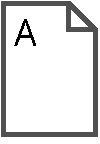
\includegraphics[scale=0.5]{fig/collab/doc-txt-a.pdf}}
            ](A){
\includegraphics[scale=0.6]{collab/device.pdf}}
            to +(70:2) node[
                label=above:{Bea},
                label=right:{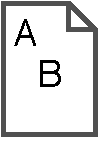
\includegraphics[scale=0.5]{fig/collab/doc-txt-ab.pdf}}
            ](B){
\includegraphics[scale=0.6]{collab/device.pdf}}
            to +(-50:2) node[
                label=below:{Carol},
                label=right:{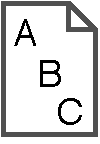
\includegraphics[scale=0.5]{fig/collab/doc-txt-abc.pdf}}
            ](C){
\includegraphics[scale=0.6]{collab/device.pdf}};
        % Links
        \draw[link] (A) to (B);
        \draw[link,-latex] (C) to node[midway]{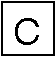
\includegraphics[scale=0.5]{fig/collab/msg-txt-c.pdf}} (B);
        \draw[link,-latex] (C) to node[midway]{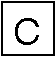
\includegraphics[scale=0.5]{fig/collab/msg-txt-c.pdf}} (A);
    \end{tikzpicture}
    \caption{}\label{fig:op-integration-order-example-1}
\end{subfigure}%
\begin{subfigure}{.5\linewidth}
\centering
    \begin{tikzpicture}
        % devices
        \path (0,0)
            to +(190:2) node[
                label=below:{Alice},
                label=left:{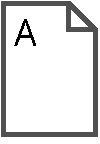
\includegraphics[scale=0.5]{fig/collab/doc-txt-a.pdf}}
            ](A){\includegraphics[scale=0.6]{collab/device.pdf}}
            to +(70:2) node[
                label=above:{Bea},
                label=right:{\includegraphics[scale=0.5]{fig/collab/doc-txt-abc.pdf}}
            ](B){\includegraphics[scale=0.6]{collab/device.pdf}}
            to +(-50:2) node[
                label=below:{Carol},
                label=right:{\includegraphics[scale=0.5]{fig/collab/doc-txt-abc.pdf}}
            ](C){\includegraphics[scale=0.6]{collab/device.pdf}};
        % Links
        \draw[link] (A) to (B);
        \draw[link] (B) to (C);
        \draw[link] (C) to (A);
    \end{tikzpicture}
    \caption{}\label{fig:op-integration-order-example-2}
\end{subfigure}
\caption[Intégration causale d'une opération]{Exemple d'intégration causale d'une opération.
Un ensemble de pairs réplique un texte.
La synchronisation des copies reposent sur une livraison causale des modifications.
\subref{fig:op-integration-order-example-1} Carol insère le caractère $\textsc{'C'}$ à sa copie qui intégré déjà les caractères $\textsc{'A'}$ et $\textsc{'B'}$.
Elle propage sa modification a Alice et Bea.
Pour intégrer le caractère $\textsc{'A'}$ sur une copie, la copie doit déjà contenir les caractères $\textsc{'A'}$ et $\textsc{'B'}$.
Alice n'a pas reçu l'insertion du caractère $\textsc{'B'}$.
Elle ne peut donc pas insérer le caractère $\textsc{'C'}$.
Elle retarde l'intégration de cette modification jusqu'à la réception du caractère $\textsc{'B'}$.
En revanche, la copie de Bea contient déjà les caractères $\textsc{'A'}$ et $\textsc{'B'}$.
\subref{fig:op-integration-order-example-2} Elle intègre donc la modification de Carol.
}\label{fig:op-integration-order-example}
\end{figure}

Généralement, ces protocoles supportent par conception l'édition hors-ligne et en sous-groupes déconnecté·e·s les uns des autres.
Cependant, lorsque les périodes de déconnexion sont longues ou le nombre de modifications hors ligne est important, la synchronisation est coûteuse en communication et en ressources de calcul.
En effet, chaque opération est transmise et intégrée aux copies des pairs.

\paragraph{}Ce qui nous amène à la deuxième question de recherche que nous explorons dans ce manuscrit~: \textbf{Est-il possible de concevoir un protocole de réplication optimiste pour l'édition collaborative de texte en simultané qui intègre immédiatement toute modification et est adapté aux longues périodes de déconnexions~?}

\paragraph{}A notre connaissance, la synchronisation par opérations est le seul schéma de synchronisation utilisé pour l'édition collaborative de texte en simultané.
D'autres schémas de synchronisation ont été proposés pour la conception de protocole de réplication.
La synchronisation par états~\autocite{shapiro_2011_crdt} consiste à transmettre l'état de la copie une fois mise à jour au lieu d'une opération.
Les états sont fusionnés de telle sorte à inclure les mise-à-jours de chacun.
Ce schéma tire son avantage principal du fait qu'un état synthétise l'ensemble des modifications qui ont été précédemment intégrées.
Les états peuvent donc être livrés et intégrés plusieurs fois dans des ordres arbitraires.
Ce qui implique qu'ils peuvent être dupliqués, omis, et réordonnés par le réseau sans compromettre la convergence des copies.
Les pairs peuvent donc intégrer un état dès sa réception.
Il n'y a pas d'intégration retardée d'états.
Par ailleurs, le système est moins sensible aux longues périodes de déconnexions des pairs.
Au lieu de transmettre une longue liste d'opérations, les pairs transmettent simplement l'état de leur copie.

Malgré ces avantages, le schéma de synchronisation par états est resté circonscrit à un petit nombre de protocoles de réplication.
Le schéma implique en effet un coût en communication et en fusion important lorsque les états sont de taille importante.
C'est le cas des copies de contenu textuel.
En effet, il n'est pas raisonnable de transmettre et intégrer l'état d'un document chaque fois qu'un caractère est inséré ou supprimé du document.

Un schéma de synchronisation par différences d'états~\autocite{almeida_2018_delta-crdt-revisited} a récemment été proposé pour tenter de réduire le coût du schéma de synchronisation par états.
Ce schéma autorise toujours la transmission d'états complets.
Cependant, il privilégie l'envoie de différences d'états qui synthétisent une ou plusieurs modifications.
Les différences d'états peuvent être intégrées plusieurs fois dans des ordres arbitraires.
Le schéma de synchronisation par différences d'états offre ainsi de nombreuses possibilités dans la manière de synchroniser deux copies.
Par exemple, lorsque des pairs collaborent en simultané ils peuvent échanger des différences d'états, alors que deux pairs qui se reconnectent après une longue période de déconnexion peuvent échanger directement leur état.

%Contrairement à la synchronisation par opérations, la synchronisation par différences d'états ne retardent pas l'intégration de modification.
%Elle ne propage donc pas de latence dans l'ensemble du système.
%Par ailleurs, sa flexibilité permet de synchroniser deux pairs par l'échange de leur état respectif.
%Lorsque deux pairs se reconnectent après une longue période de déconnexion, ils n'ont pas besoin d'échanger leurs modifications une à une.
%Ils peuvent directement transmettre leur état.
Nous proposons d'adopter ce schéma de synchronisation pour l'édition collaborative de texte.
Pour ce faire, nous concevons un nouveau protocole de réplication optimiste nommé \emph{Dotted LogootSplit}.


\section{Organisation du manuscrit}

Le reste du manuscrit est organisé en 5 chapitres~:

\paragraph{Le \autoref{ch:problematic}} introduit plus en détail les caractéristiques des infrastructures pair-à-pair de collaboration et met l'accent sur les problématiques de recherche liées à la convergence des copies et à sa protection. Le chapitre définit également l'adversaire du système qui contrôle les pairs mal-intentionnés.

\paragraph{Le \autoref{ch:background}} présente les formalismes que nous utilisons dans les chapitres suivants pour décrire nos contributions.
Nous introduisons en particulier la notion de cohérence de données et les types de données répliqués.

%\paragraph{Le \autoref{ch:secured-convergence}} présente notre première contribution qui propose de diviser en deux sous-classes : les \acp{CRDT} étiquetés et les \acp{CRDT} non-étiquetés. Nous montrons que la convergence des \acp{CRDT} non-étiquetés est protéger par conception ou peut être protégé en utilisant un journal authentifié. Nous proposons un mécanisme pour protéger les \acp{CRDT} étiquetés synchronisé par opérations.

\paragraph{Le \autoref{ch:pruned-log}} présente deux protocoles qui protègent la convergence des copies des pairs honnêtes.
Le protocole à journaux complets protège la convergence des copies des pairs honnêtes à l'aide de journaux authentifiés et complets.
Le protocole à journaux tronqués repose sur le protocole à journaux complets.
Il permet la troncature des journaux et l'authentification de l'état d'une copie à l'aide d'un journal tronqué.
Pour développer ce protocole, le chapitre introduit la notion de stabilité et \emph{DynVFJC}, un nouveau modèle de cohérence.
%notre mécanisme pour tronquer un journal authentifié. Nous développons \emph{DynVFJC} un modèle de cohérence de donnée basé sur \acl{VFJC} qui permet de stabiliser un journal authentifié dans un groupe dont la composition évolué au cours du temps et qui peut inclure des pairs mal-intentionnés. Nous présentons également \acl{VFJCS} qui définit qu'elle partie du journal est stable.
Nous présentons également les travaux de la littérature en relation avec notre protocole.

\paragraph{Le \autoref{ch:dotted-logootsplit}} présente un état de l'art des types séquences de données répliquées.
Nous proposons un modèle unifié pour décrire et mieux appréhender un sous-ensemble de ces types séquence.
A l'aide de ce modèle nous répondons à notre deuxième question de recherche en proposant \emph{Dotted LogootSplit}, le premier type séquence de données répliquées synchronisé par différence d'états.

\paragraph{Le \autoref{ch:conclusion}} clôt ce manuscrit et propose des axes d'exploration pour continuer les travaux de recherche présentés au sein de ce manuscrit.


\section{Publications}

La première contribution développée au sein de ce manuscrit a fait l'objet d'une publication~\autocite{2018_elvinger_prunable-auth-log}.
La seconde contribution présentée n'a pas encore fait l'objet d'une publication.
En revanche, la proposition a été implémentée dans notre prototype d'éditeur collaboratif \emph{MUTE} qui est décrit dans l'une de nos publications~\autocite{2017_nicolas-mute-demo}.
Notre dernière publication~\autocite{2019_yu_genericundo} est en lien avec nos travaux sur les type de données répliquées, mais n'est pas présentée au sein de ce manuscrit.
Dans la suite de cette section nous référençons les articles qui ont été publiés au cours de cette thèse.

\subsection*{Prunable Authenticated Log and Authenticable Snapshot in Distributed Collaborative Systems \autocite{2018_elvinger_prunable-auth-log}}

-- Victorien Elvinger, Gérald Oster, François Charoy

\paragraph{Article de conférence} in proceedings of the 4th {IEEE} International Conference on Collaboration and Internet Computing, ({CIC} 2018)

\paragraph{Abstract:} In distributed collaborative systems, participants maintain a replicated copy of shared documents.
They edit their own copy and then share their modifications without any coordination.
Copies follow successions of divergence and convergence.
Convergence is a liveness property of collaborative systems.
Some malicious participants may find an advantage to make the collaboration fail. 
To that end, they can preclude convergence of the copies.
%
To protect convergence of copies, participants can exploit an authenticated log of modifications.
New participants have to retrieve the entire log in order to contribute. Unfortunately, the cost of joining a collaboration increases with the size of this log.
Causal Stability allows to prune authenticated logs in a static collaborative group without any malicious participants.
%
In this paper, we first tailor Causal Stability to dynamic groups in presence of malicious participants.
We then propose a mechanism to verify the consistency of a pruned log and a mechanism to authenticate a snapshot from a pruned log.

\bigskip
\bigskip

\subsection*{MUTE\@: A Peer-to-Peer Web-based Real-time Collaborative Editor \autocite{2017_nicolas-mute-demo}}

-- Matthieu Nicolas, Victorien Elvinger, Gérald Oster, Claudia-Lavinia Ignat,
François Charoy

\paragraph{Article de démonstration} in proceedings of the 15th European Conference on Computer Supported Cooperative Work ({ECSCW} 2017)

\paragraph{Abstract:} Real-time collaborative editing allows multiple users to edit shared documents at the same time from different places. Existing real-time collaborative editors rely on a central authority that stores user data which is a perceived privacy threat. In this paper, we present \acf{MUTE}, a peer-to-peer web-based real-time collaborative editor without central authority disadvantages. Users share their data with the collaborators they trust without having to store their data on a central place. MUTE features high scalability and supports offline and ad-hoc collaboration.

\clearpage

\subsection*{A Generic Undo Support for State-Based CRDTs \autocite{2019_yu_genericundo}}

-- Weihai Yu, Victorien Elvinger, Claudia-Lavinia Ignat

\paragraph{Article de conférence} in proceedings of the 23rd International Conference on Principles of Distributed Systems, ({OPODIS} 2019)

\paragraph{Abstract:} CRDTs (Conflict-free Replicated Data Types) have properties desirable for large-scale distributed systems with variable network latency or transient partitions.
With CRDT, data are always available for local updates and data states converge when the replicas have incorporated the same updates.
Undo is useful for correcting human mistakes and for restoring system-wide invariant violated due to long delays or network partitions.
There is currently no generally applicable undo support for CRDTs.
There are at least two reasons for this. First, there is currently no abstraction that we can practically use to capture the relations between undo and normal operations with respect to concurrency and causality. 
Second, using inverse operations as the existing partial solutions, the CRDT designer has to hard-code certain rules and design a new CRDT for almost every operation that needs undo support.
In this paper, we present an approach to generic support of undo for CRDTs. The approach consists of two major parts.
We first work out an abstraction that captures the semantics of concurrent undo and redo operations through equivalence classes.
The abstraction is a natural extension of undo and redo in sequential applications and is straightforward to implement in practice.
By using this abstraction, we then device a mechanism to augment existing CRDTs.
The mechanism provides an ``out of the box'' support for undo without the involvement of the CRDT designers.
We also present a practical application of the approach in collaborative editing.



%\section{Infrastructures de collaboration}
%\vicnote{A intégrer dans l'intro}
%
%% flux d'activité = collaborateur + dimension temporel
%
%% mode de collaboration et infras
%Les infrastructures de collaboration permettent à des groupes de collaborateur·ice·s de produire collectivement des contenus.
%Elles restreignent les formes que peuvent prendre ces collaborations.
%Par exemple, l'encyclopédie Wikipedia et le gestionnaire de versions SVN permettent uniquement la modification exclusive d'un contenu ou d'un sous-ensemble d'un contenu.
%Le contenu ne peut être modifié que par un·e seul·e utilisateur·ice à la fois.
%Des gestionnaires de versions distribués comme Git ou Mercurial permettent à plusieurs utilisateur·ice·s de modifier simultanément, mais de manière asynchrone, un même contenu.
%Les utilisateur·ice·s modifient les contenus et se synchronisent à posteriori avec les autres.
%Les éditeurs de textes collaboratifs comme Etherpad ou Goggle Docs permettent à leurs utilisateur·ice·s de modifier simultanément et de manière synchrone un contenu.
%Les utilisateur·ice·s ont l'illusion d'observer les modifications des autres en temps réel.
%\vicnote{Détailler chaque mode de collaboration ?}
%
%En l'absence de restrictions imposées par des infrastructures de collaboration, une activité de collaboration peut prendre différentes formes en fonction des individus et évoluer au cours du temps.
%Reconsidérons l'exemple de l'écriture collaborative d'un logiciel. Des programmeur·euse·s peuvent vouloir modifier de manière isolé une partie du logiciel et se synchroniser à posteriori avec les autres.
%Cette isolation leur permet d'évaluer avec plus de précision l'effet de leurs modifications sur une suite de tests logiciels.
%En revanche, d'autres programmeur·euse·s, éventuellement les mêmes mais à un autre moment, désirent peut être programmer en binômes isolés communément appelé \emph{pair programming}.
%Chaque membre d'un binôme travaille simultanément et de manière synchrone sur un même fichier.
%Cette exemple illustre la diversité des activités de collaboration qui peuvent avoir lieu au sein d'une même équipe qui produit collectivement un contenu.
%Cette composition des modes synchrone et asynchrone est nommée \emph{multi-synchrone} dans la littérature~\autocite{dourish_1995_divergence}.
%
%\vicnote{illustration}
%
%%Les infrastructures traditionnels de collaboration supportent un sous-ensemble des modes d'organisation.
%Les infrastructures traditionnelles de collaboration supportent généralement un sous-ensemble des formes de collaboration.
%Git et Mercurial ne permettent pas une collaboration synchrone.
%Seules les formes asynchrones sont possibles.
%Etherpad et Google Docs ne permettent pas de contribuer à un contenu de manière isolé.
%Les collaboration synchrone requiert une latence faible pour produire l'illusion d'une collaboration en temps réel.
%Elle ne tolère pas les partitions réseaux.
%En revanche les collaboration asynchrone sont tolérantes aux délais, aux pannes, et aux partitions réseaux.
%Elles passent facilement à l'échelle.
%
%% infra P2P
%Les infrastructures pair-à-pair de collaboration ont été conçues pour permettre les collaborations multi-synchrones.
%
%AUTRE EXEMPLES : Nuit debout, télétravail / cours durant la crise du Covid 19.

% BD distribué, DVCS, éditeurs collaboratifs
